\documentclass{article}

\usepackage{arxiv}

\usepackage[utf8]{inputenc} % allow utf-8 input
\usepackage[T1]{fontenc}    % use 8-bit T1 fonts
\usepackage{lmodern}        % https://github.com/rstudio/rticles/issues/343
\usepackage{hyperref}       % hyperlinks
\usepackage{url}            % simple URL typesetting
\usepackage{booktabs}       % professional-quality tables
\usepackage{amsfonts}       % blackboard math symbols
\usepackage{nicefrac}       % compact symbols for 1/2, etc.
\usepackage{microtype}      % microtypography
\usepackage{lipsum}
\usepackage{graphicx}

\title{A linear modelling exploration of predictors of scores in the AFL}

\author{
    Trent Henderson
   \\
    OLET5608 \\
   \\
  \texttt{\href{mailto:then6675@uni.sydney.edu.au}{\nolinkurl{then6675@uni.sydney.edu.au}}} \\
  }


% Pandoc citation processing



\begin{document}
\maketitle

\def\tightlist{}


\begin{abstract}
AFL is a highly-popular Australian sport that has garnered a lot of talk
show attention, but suffers from a lack of statistical rigour. The
present report sought to bridge this gap by providing a statistically
robust exploration of predictors of scoring using data aggregated at the
team and match level. A regression approach was adopted, which comprised
an ordinary least squares and generalised additive model. Results found
that hit outs and contested marks did not significantly predict scoring,
while tackles and unforced errors singificantly and negatively predicted
scoring, and rebounds, marks inside 50, marks, inside 50s, handballs,
free kicks for, contested possessions, and clearances all significantly
and positively predicted scoring. Implications for coaching and gameplay
strategy, as well as limitations are discussed.
\end{abstract}


\hypertarget{introduction}{%
\section{Introduction}\label{introduction}}

AFL is a highly popular Australian sports league that began in 1896 and
continues strongly today, with Grand Final match attendance (outside of
the anomalous COID-19-impacted 2020 season) approximating a sold out
100,000 each year at the traditional host venue - the Melbourne Cricket
Ground. An AFL match is won based on points, which can be accumulated by
kicking either a goal (worth six points) or a behind (worth one point).
Despite its popularity and complexity, AFL is a sport that has
traditionally relied on subject matter expertise and the knowledge of
past players to inform coaching strategies. Much like other Australian
sports, a lack of empirical statistical sophistication is evident.

Globally, sport analytics has continued to generate increasing
attention, with websites such as FiveThirtyEight and Advanced Sports
Analytics creating stylish platforms that constitute a reliable source
of insight and interactive analysis. However, this form of innovative
and detailed sports analytics has yet to fully breach Australian sports.
While the AFL has dedicated talk show analysis television programs such
as AFL 360, The Front Bar, and Talking Footy, these programs focus
mostly on qualitative breakdowns of high-level match statistics and not
on statistical rigour. This report aims to bridge some of this gap by
providing a preliminary statistical investigation of factors associated
with scoring in the AFL. Specifically, this report aims to explore the
following research question: \emph{Which gameplay attributes are
predictors of scores in AFL matches?}

\hypertarget{data-set}{%
\section{Data set}\label{data-set}}

Historical AFL data has been made readily-accessible in an open-source
setting through the R package \texttt{fitzRoy} (see Day, Nguyen, and
Lane 2020). The package provides a simple API that accesses and
integrates a range of data sources that collate AFL data. Examples of
these sources include:

\begin{itemize}
  \item{AFL}
  \item{AFL Tables}
  \item{Squiggle}
  \item{FootyWire}
\end{itemize}

The data itself is diverse, covering domains as broad as player and
match statistics, Brownlow medal votes, betting odds, attendance
numbers, and match times. This report focuses on player and match
statistics by aggregating quantities of interest to team-per-match-level
sums using data for the 2005-2019 seasons, inclusive. This time period
is partially arbitrary, but was made on the basis of recency and
potential homogeneity. The 2020 season is a strong counter example of
this where the season length was truncated and played almost entirely in
Queensland due to the impacts of COVID-19. This means the standard set
up of games - having a home and away team - was not normal in 2020 and
thus data for the entire season may represent a heterogenous set.

\hypertarget{data-limitations}{%
\subsection{Data limitations}\label{data-limitations}}

Despite the availability of so much player-level data, the author of the
\texttt{fitzRoy} package and the creators of the sources it pulls from
(listed above) all note potential caveats around their data. The main
caveat is that the data is not official. Each source pulls from multiple
others, and many individual people are involved in the continual
updating of information. The accuracy of the data in \texttt{fitzRoy} is
largely contingent on the accuracy of the sources underpinning the
websites it scraped. While this is cause for concern, there are a large
number of industry-standard sources that comprise the majority of the
data used in this report, including official statistics produced by the
AFL, newspapers and magazines (such as The Herald Sun and Inside
Football), and official books (such as Main and Holmesby (2018) and
Rodgers (1996)). The open-source nature of many of the sources,
especially AFL Tables, means continual improvement and accuracy is being
achieved, further lending confidence to the available data.

\hypertarget{variable-retention}{%
\subsection{Variable retention}\label{variable-retention}}

A small subset of variables were retained from the much larger dataset.
The subset was developed based on the author's subject matter expertise
of AFL. The variables retained were selected based on their likely
relationship to a team's ability to score and whether a team could
implement a training or coaching intervention off the back of this
analysis to better target the predictors. For example, the variable
\emph{free kicks against} was not included, as the number of free kicks
given away by a team is not a core contributor to the same team scoring,
and it is likely near impossible to coach out of the game.

The variables that were retained for the purposes of this analysis
included team-match-level counts of scores, marks, handballs, hit outs,
tackles, rebounds, inside 50s, clearances, clangers (unforced errors),
free kicks for, contested possessions, contested marks, and marks inside
50.

\hypertarget{analysis}{%
\section{Analysis}\label{analysis}}

A rigorous and detailed linear modelling pipeline was implemented. This
involved the following steps, each of which will be discussed in turn:

\begin{enumerate}
\def\labelenumi{\arabic{enumi}.}
\tightlist
\item
  Exploratory data analysis and visualisation
\item
  Model fitting
\item
  Model assumption testing
\item
  Model re-specification (if required)
\item
  Model interpretation
\item
  Preliminary advanced model exploration
\end{enumerate}

\hypertarget{exploratory-data-analysis-and-visualisation}{%
\subsection{Exploratory data analysis and
visualisation}\label{exploratory-data-analysis-and-visualisation}}

Prior to modelling, the data were aggregated and explored visually and
numerically to understand the empirical structure. The data was
aggregated to match-level sums for each time by summing over individual
player statistics. Figure @ref(fig:distplot) below shows the
distributions of each aggregated quantitative variable.

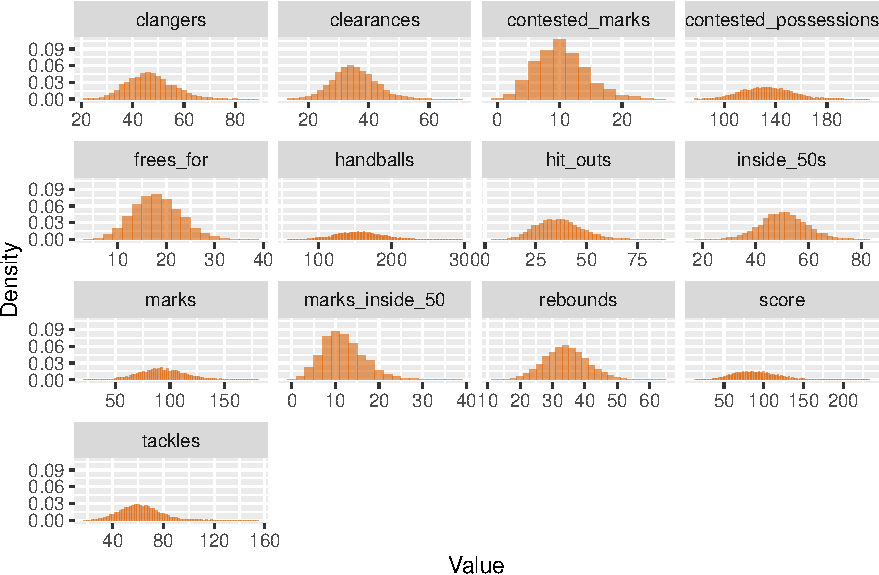
\includegraphics{OLET5608_TrentHenderson_files/figure-latex/distplot-1.pdf}

The data were further explored using high-level summary statistics.
These are presented below in Table @ref(tab:summarystats). Note the
large difference in scales between the variables. To avoid issues with
high-variance predictors influencing linear modelling or producing
extremely low coefficients, all predictors were mean-centred and
standardised (z-scored) prior to modelling. This also means the
coefficients will have an intuitive interpretation compared to other
rescaling methods.

\% latex table generated in R 4.0.2 by xtable 1.8-4 package \% Thu May 6
16:40:45 2021

\begin{table}[ht]
\centering
\begin{tabular}{rl}
  \hline
 & type \\ 
  \hline
1 & numeric \\ 
   \hline
\end{tabular}
\end{table}

\hypertarget{model-fitting}{%
\subsection{Model fitting}\label{model-fitting}}

\hypertarget{model-assumption-testing}{%
\subsection{Model assumption testing}\label{model-assumption-testing}}

There are four core assumptions of linear regression model (see Faraway
2004). These include:

\begin{enumerate}
\def\labelenumi{\arabic{enumi}.}
\tightlist
\item
  Linear relationship between \texttt{X} and \texttt{y}
\item
  Independent observations
\item
  Homogeneity of variance
\item
  Normality of residuals
\end{enumerate}

Since it is known that the data used for this report are independent
observations, the following sections will focus on reporting the testing
of the other assumptions.

\hypertarget{assumption-1-linear-relationship}{%
\subsubsection{Assumption 1: Linear
relationship}\label{assumption-1-linear-relationship}}

The purpose of a linear model is to understand the relationship between
some number of predictors and a quantitative response variable. As such,
a linear model at its core assumes that all predictors are related
linearly to the response variable.

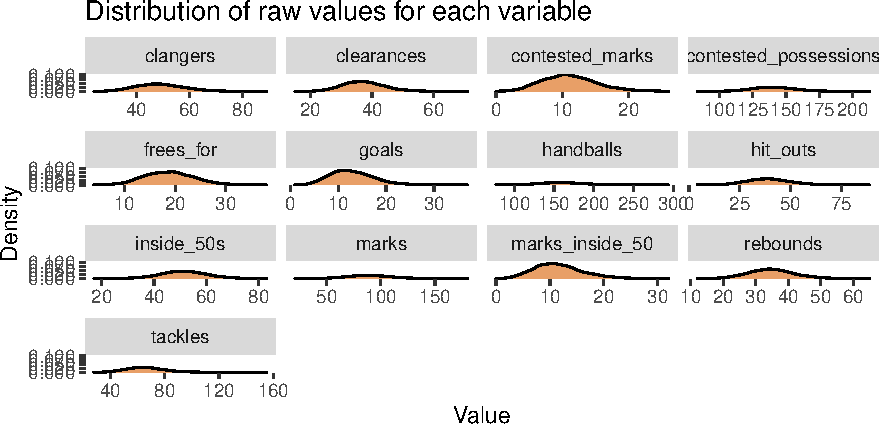
\includegraphics{OLET5608_TrentHenderson_files/figure-latex/unnamed-chunk-4-1.pdf}

A secondary visual test was conducted with a robust regression (using
M-estimation) as the plots above appeared to contain some potential
leverage points or outliers. The plot has been omitted for space,
however there was almost no visual difference between the standard
linear and the robust linear approaches.

While all variables were being tested for appropriateness, a variance
inflation factor (VIF) test was undertaken to estimate potential
multicollinearity between the predictors. Multicollinearity is an issue
as it can drive imprecise estimates, change parameter value signs, and
impact \(R^2\) (see Hair et al. 2010). Different threshold values exist
for the VIF, with cutoffs ranging from values less than four being
acceptable (see Hair et al. 2010) to values less than ten being
acceptable (see Hair et al. 1995). Outputs from the VIF test are
presented below in Table @ref(tab:vif). Evidently, no predictor violates
even the lowest bound commonly cited in the literature, indicating no
issue with multicollinearity.

\begin{verbatim}
##                Variables Tolerance      VIF
## 1                  marks 0.5683153 1.759587
## 2              handballs 0.7913858 1.263606
## 3               hit_outs 0.6969646 1.434793
## 4                tackles 0.6600943 1.514935
## 5               rebounds 0.7584166 1.318537
## 6             inside_50s 0.5373581 1.860956
## 7             clearances 0.4959750 2.016231
## 8               clangers 0.7910878 1.264082
## 9              frees_for 0.9075108 1.101915
## 10 contested_possessions 0.3002560 3.330491
## 11       contested_marks 0.7390768 1.353039
## 12       marks_inside_50 0.5687182 1.758340
\end{verbatim}

\hypertarget{assumption-2-homogeneity-of-variance}{%
\subsubsection{Assumption 2: Homogeneity of
variance}\label{assumption-2-homogeneity-of-variance}}

Homoegeneity of variance - the lack of a systematic pattern or bias of
residuals across model fitted or predictor values - is another core
linear model assumption. This assumption is typically assessed
graphically using a residuals plot, where fitted values are plotted
against model residuals. A model with homogeneity of variance should
have no discernible pattern across the fitted values. This plot is
depicted in the upper left in the graphics matrix below.

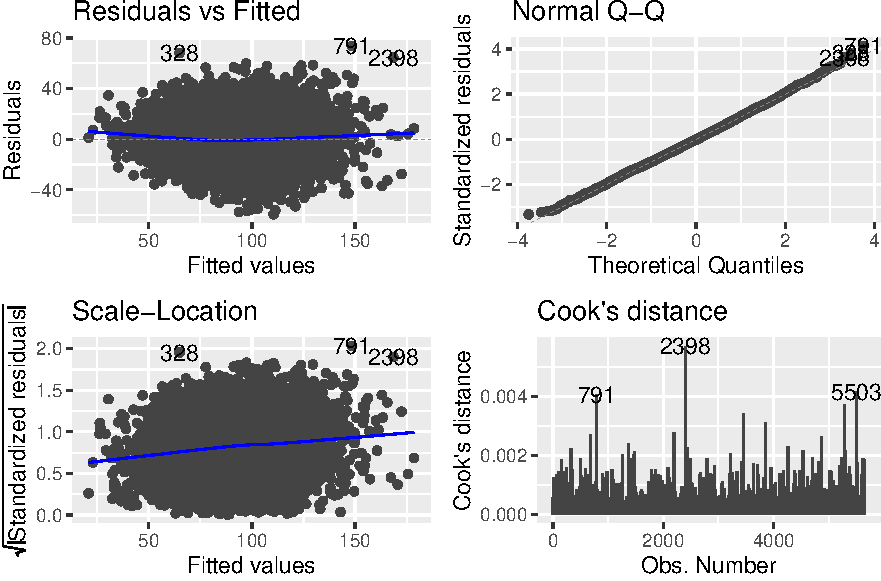
\includegraphics{OLET5608_TrentHenderson_files/figure-latex/unnamed-chunk-5-1.pdf}

Evidently, there is a slight sag in the line through this plot,
indicating potential heteroscedasticity. It was first hypothesised that
potential outliers might be influencing the results, despite the lack of
compelling visual evidence based on the Cook's Distance plot. Following
advice from (Faraway 2004), a test of the maximum studentised residual
value against a Bonferroni-corrected critical value. Since the maximum
residual value of 4.14 was less than the critical value of 4.45, it was
declared that outliers were not a major issue.

\hypertarget{assumption-3-normality-of-residuals}{%
\subsubsection{Assumption 3: Normality of
residuals}\label{assumption-3-normality-of-residuals}}

Normality of residuals is typially assessed graphically using a Q-Q
plot, as seen in the upper right graphic in the matrix presented above.
A model with normally-distributed residuals should lie directly on the
diagonal line. The residuals are almost entirely positioned on the line
with very little variation at the ends indicating no issues with
normality.

\hypertarget{preliminary-advanced-model-exploration}{%
\subsection{Preliminary advanced model
exploration}\label{preliminary-advanced-model-exploration}}

One other model was fit in addition to the standard linear model - a
generalised additive model (GAM) (see Hastie and Tibshirani 1986). GAMs
further generalise the commonly-used generalised linear model (GLM) to
greatly increase flexibility and potential to model non-linearities.
GAMs achieve this through the use of splines and basis functions whose
number is specified by a knot parameter, and which are connected by
smoothed polynomials. GAMs essentially enable the fitting of wiggly
functions over the data with parameter optimisation. The basic form of a
GAM is written in Equation @ref(eq:gam), where the predictors are still
entered linearly, but they are instead modelled using some unknown
smooth functions:

\begin{equation}
y_i = \beta_0 + f_1(x_i) + f_2(x_i)... + f_n(x_n) + \epsilon_i (\#eq:gam)
\end{equation}

Where \(\epsilon\) is (in the standard linear modelling case) Gaussian
noise \(\mathcal{N}(\mu,\sigma^2)\), specified by its mean and standard
deviation. Of course, similar to GLMs, this Gaussian noise assumption is
generalised to other probability distributions, though these are not the
considered in this report. The GAM for this report was fit in \texttt{R}
using the \texttt{mgcv} package (see Wood 2011). It was fit using
Restricted Maximum Likelihood for reduced-rank model parameter
estimation, as per advice by Wood (see Wood, n.d.).

\hypertarget{model-assumption-testing-1}{%
\subsubsection{Model assumption
testing}\label{model-assumption-testing-1}}

Similar to the standard linear model, core assumptions still need to
hold for the GAM. These were also tested, with a summary output
presented below in Figure @ref(fig:gamvis) generated by the \texttt{R}
package \texttt{mgcViz} (see Fasiolo et al. 2018).

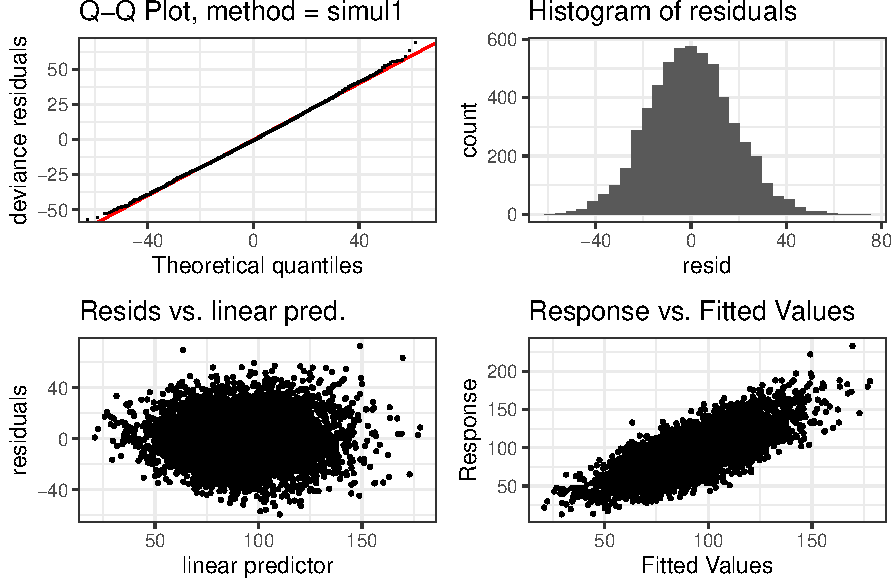
\includegraphics{OLET5608_TrentHenderson_files/figure-latex/gamvis-1.pdf}

\hypertarget{results}{%
\section{Results}\label{results}}

The results section is organised by model type. Results for the linear
model are discussed first, followed by the generalised additive model.

\hypertarget{linear-model}{%
\subsection{Linear model}\label{linear-model}}

Mean estimates and 95\% confidence intervals for each coefficient is
presented below in Figure @ref(fig:coefs).

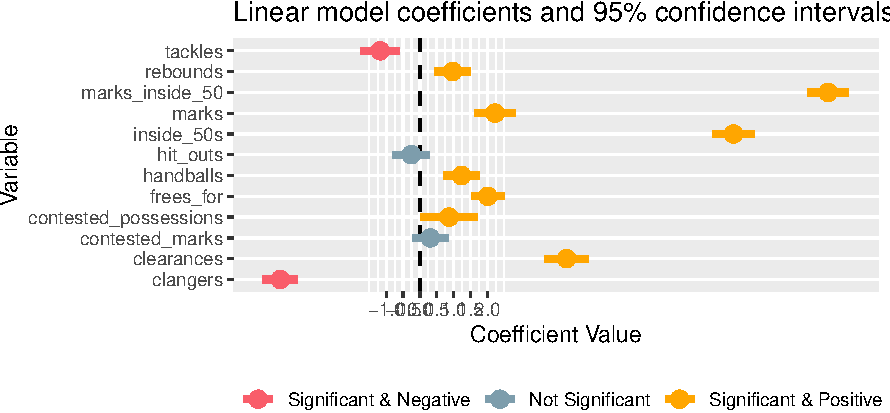
\includegraphics{OLET5608_TrentHenderson_files/figure-latex/coefs-1.pdf}

A more detailed numerical presentation of coefficients is depicted below
in Table @ref(tab:coeftable). Since all predictors were mean-centred and
standardised (z-scored) prior to analysis, the interpretation is as
follows: \emph{the coefficient represents the change in total score
(response variable) for a one standard deviation change (increase or
decrease, depending on sign of the coefficient) in the predictor}. The
results table below also contains information regarding the overall
model fit and \emph{F}-statistic. The overall model is statistically
significant, \emph{F} = 676.7 (\emph{df} = 12; 5639), and explains
approximately 58.9\% of the observed variance in scores.

\begin{table}[!htbp] \centering 
  \caption{} 
  \label{} 
\begin{tabular}{@{\extracolsep{5pt}}lc} 
\\[-1.8ex]\hline 
\hline \\[-1.8ex] 
 & \multicolumn{1}{c}{\textit{Dependent variable:}} \\ 
\cline{2-2} 
\\[-1.8ex] & score \\ 
\hline \\[-1.8ex] 
 marks & 2.233$^{***}$ \\ 
  & (0.315) \\ 
  & \\ 
 handballs & 1.238$^{***}$ \\ 
  & (0.267) \\ 
  & \\ 
 hit\_outs & $-$0.257 \\ 
  & (0.284) \\ 
  & \\ 
 tackles & $-$1.179$^{***}$ \\ 
  & (0.292) \\ 
  & \\ 
 rebounds & 0.974$^{***}$ \\ 
  & (0.273) \\ 
  & \\ 
 inside\_50s & 9.318$^{***}$ \\ 
  & (0.324) \\ 
  & \\ 
 clearances & 4.358$^{***}$ \\ 
  & (0.337) \\ 
  & \\ 
 clangers & $-$4.148$^{***}$ \\ 
  & (0.267) \\ 
  & \\ 
 frees\_for & 2.020$^{***}$ \\ 
  & (0.249) \\ 
  & \\ 
 contested\_possessions & 0.866$^{**}$ \\ 
  & (0.433) \\ 
  & \\ 
 contested\_marks & 0.309 \\ 
  & (0.276) \\ 
  & \\ 
 marks\_inside\_50 & 12.129$^{***}$ \\ 
  & (0.315) \\ 
  & \\ 
 Constant & 90.267$^{***}$ \\ 
  & (0.237) \\ 
  & \\ 
\hline \\[-1.8ex] 
Observations & 5,652 \\ 
R$^{2}$ & 0.590 \\ 
Adjusted R$^{2}$ & 0.589 \\ 
Residual Std. Error & 17.852 (df = 5639) \\ 
F Statistic & 676.676$^{***}$ (df = 12; 5639) \\ 
\hline 
\hline \\[-1.8ex] 
\textit{Note:}  & \multicolumn{1}{r}{$^{*}$p$<$0.1; $^{**}$p$<$0.05; $^{***}$p$<$0.01} \\ 
\end{tabular} 
\end{table}

Evidently, both hit outs (\emph{t} = -0.91, \emph{p} = 0.366) and
contested marks (\emph{t} = 1.1, \emph{p} = 0.263) were the only two
non-significant predictors. Of the remaining predictors, two were
negative and statistically significant. These included tackles (\emph{t}
= -4.0, \emph{p} \textless{} .001) and clangers (\emph{t} = -15.5,
\emph{p} \textless{} .001), such that a one standard deviation increase
in tackles is associated with mean reduction of 1.2 in total score,
while a one standard deviation increase in clangers is associated with
mean reduction of 4.1 in total score. On the positive predictors, the
two with the strongest coefficients are also conceptually related:
inside 50s (\emph{t} = 28.76, \emph{p} \textless{} .001) and marks
inside 50 (\emph{t} = 38.51, \emph{p} \textless{} .001). The magnitude
of both these predictors is noteworthy, as a one standard deviation
increase in inside 50s is associated with a mean increase of 9.3 in
total score, and a one standard deviation increase in marks inside 50 is
associated with a mean increase of 12.1 in total score.

\hypertarget{gam}{%
\subsection{GAM}\label{gam}}

Coefficient plots for each predictor are presented below in Figure
@ref(fig:gamsmooths). Thhe interpretation relative to the standard
linear model is important and interesting.

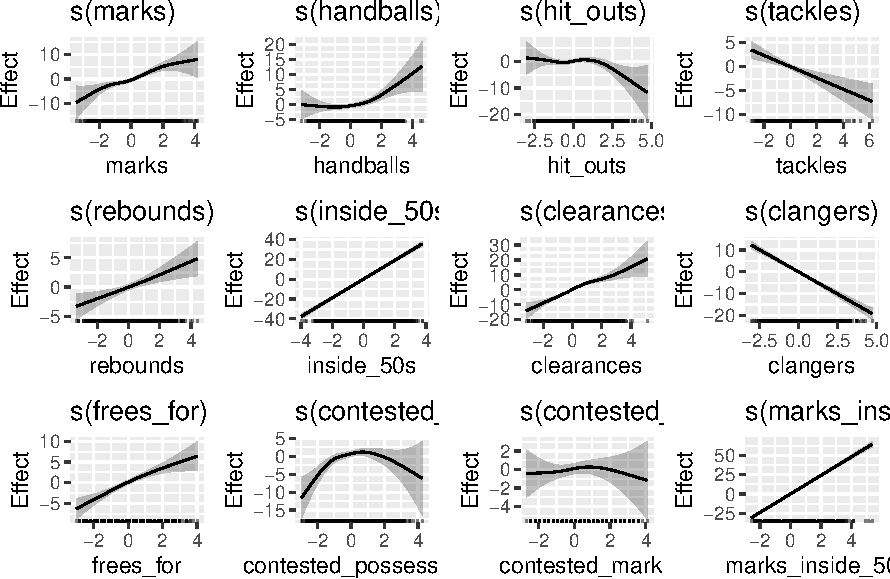
\includegraphics{OLET5608_TrentHenderson_files/figure-latex/gamsmooths-1.pdf}

A detailed numerical presentation of coefficients is depicted below in
Table @ref(tab:gamcoefs). The interpretation of smooth coefficients is
different from that of the ordinary least squares model.

\hypertarget{comparison-to-linear-model}{%
\subsubsection{Comparison to linear
model}\label{comparison-to-linear-model}}

The GAM clearly adds complexity to the model. To compare the efficacy of
the GAM with the standard ordinary least squares model, a metric that
penalises complexity must be used, as parsimony is to be strived toward
in statistical analysis to avoid overfitting. The Akaike information
criterion (AIC) and Bayesian information criterion (BIC) are two
quantities typically used for this purpose (see Posada and Buckley
2004), where the penalty for additional parameters is larger in BIC. The
results of both quantities for each model is presented below in Table
@ref(tab:penalties).

\hypertarget{discussion}{%
\section{Discussion}\label{discussion}}

The present analysis aimed to produce an innovative and statistically
robust exploration of predictors of scoring in the AFL using
team-per-match-level data.

\hypertarget{limitations}{%
\subsection{Limitations}\label{limitations}}

Variable selection

\hypertarget{references}{%
\section*{References}\label{references}}
\addcontentsline{toc}{section}{References}

\hypertarget{refs}{}
\leavevmode\hypertarget{ref-fitzRoy}{}%
Day, James, Robert Nguyen, and Oscar Lane. 2020. \emph{FitzRoy: Easily
Scrape and Process Afl Data}.
\url{https://CRAN.R-project.org/package=fitzRoy}.

\leavevmode\hypertarget{ref-R:Faraway:2004}{}%
Faraway, Julian J. 2004. \emph{Linear Models with R}. Chapman \&
Hall/CRC. \url{http://www.maths.bath.ac.uk/\%20jjf23/LMR/}.

\leavevmode\hypertarget{ref-mgcViz}{}%
Fasiolo, Matteo, Raphael Nedellec, Yannig Goude, and Simon N. Wood.
2018. ``Scalable Visualisation Methods for Modern Generalized Additive
Models.'' \emph{Arxiv Preprint}. \url{https://arxiv.org/abs/1707.03307}.

\leavevmode\hypertarget{ref-multi2}{}%
Hair, J. F., R. E. Anderson, R. L. Tatham, and W. C. Black. 1995.
\emph{Multivariate Data Analysis (3rd Ed.)}. Macmillan Publishing
Company, New York.

\leavevmode\hypertarget{ref-multi1}{}%
Hair, J. F., W. C. Black, B. J. Babin, and R. E. Anderson. 2010.
\emph{Multivariate Data Analysis (7th Ed.)}. Upper saddle River, New
Jersey: Pearson Education International.

\leavevmode\hypertarget{ref-10.1214ux2fssux2f1177013604}{}%
Hastie, Trevor, and Robert Tibshirani. 1986. ``Generalized Additive
Models.'' \emph{Statistical Science} 1 (3): 297--310.
\url{https://doi.org/10.1214/ss/1177013604}.

\leavevmode\hypertarget{ref-everyone}{}%
Main, Jim, and Russel Holmesby. 2018. \emph{The Encyclopedia of Afl
Footballers: Every Afl/Vfl Player Since 1897}. Bas Publishing.

\leavevmode\hypertarget{ref-10.1080ux2f10635150490522304}{}%
Posada, David, and Thomas R. Buckley. 2004. ``Model Selection and Model
Averaging in Phylogenetics: Advantages of Akaike Information Criterion
and Bayesian Approaches Over Likelihood Ratio Tests.'' \emph{Systematic
Biology} 53 (5): 793--808.
\url{https://doi.org/10.1080/10635150490522304}.

\leavevmode\hypertarget{ref-everygame}{}%
Rodgers, Stephen. 1996. \emph{Every Game Ever Played: VFL/Afl Results,
1897-1995}. Viking.

\leavevmode\hypertarget{ref-mgcv}{}%
Wood, S. N. 2011. ``Fast Stable Restricted Maximum Likelihood and
Marginal Likelihood Estimation of Semiparametric Generalized Linear
Models.'' \emph{Journal of the Royal Statistical Society (B)} 73 (1):
3--36.

\leavevmode\hypertarget{ref-wood}{}%
---------. n.d. ``Frequently Asked Questions for Package Mgcv.''
\url{http://web.mit.edu/~r/current/arch/i386_linux26/lib/R/library/mgcv/html/mgcv-FAQ.html}.

\bibliographystyle{unsrt}
\bibliography{references.bib}


\end{document}
